\chapterhead{3}{Answering a Question}{A model is built for some questions and not others}\label{ch3}

Every model is good at some questions and useless at others. A map can say which way to the library but not what the library smells like. A scale model can say whether a wardrobe fits an alcove but not how the wardrobe feels. Before using a model, ask: \textbf{what must this model keep to answer my question?}

\begin{center}
\sffamily\small\renewcommand{\arraystretch}{1.5}
\begin{tabular}{@{}p{3.4cm}p{3.7cm}p{3.7cm}@{}}
\toprule
\textbf{Question} & \textbf{A model that suits it} & \textbf{What it must keep}\\
\midrule
Which way to the library? & a map & places and routes\\
Will the wardrobe fit the alcove? & a scale model & sizes\\
How does blood flow round a heart? & a diagram & the order of the parts\\
\bottomrule
\end{tabular}
\end{center}

\begin{tryit}{Ask the model}
Use your $1:50$ room model from chapter~1. Write three questions about the room and predict each answer from the model alone. Then check the real room.\par\medskip
\renewcommand{\arraystretch}{1.8}
\begin{tabular}{|p{4.2cm}|p{2.8cm}|p{2.2cm}|c|}
\hline
\textbf{Question} & \textbf{Model says} & \textbf{Real room} & \textbf{Match?}\\ \hline
 & & & \\ \hline
 & & & \\ \hline
 & & & \\ \hline
\end{tabular}
\end{tryit}

\begin{worked}{Practice numbers, not from a real room}
Q1. Does the 200~cm bed fit between the desk and the end wall? The model gap is 3.8~cm, so $3.8\times50=190$~cm. The bed is 4~cm on the model. Model says: no. Real gap 190~cm. Bed 200~cm. No.\\
Q2. Does the 120~cm desk fit under the 150~cm window? Model: 2.4~cm in 3.0~cm. Model says: yes. Real: yes.\\
Q3. Does the door open fully? The model drew the door as a line with no swing. The model cannot say.
\end{worked}

\begin{center}
\begin{tikzpicture}
  \node[bigcir,minimum size=2.4cm] (a) at (0,0) {}; \node[font=\sffamily\scriptsize,align=center] at (0,0) {gap 190\\bed 200};
  \node[cir] (b) at (4.8,0) {no}; \draw[popA] (a) -- node[above,note] {bed longer than gap} (b);
  \node[note,anchor=west,text width=2.4cm,align=left] at (5.8,0) {\textbf{kept:} the two lengths\\\textbf{dropped:} door swing};
\end{tikzpicture}
\end{center}

\begin{multix}[hmm]\multixbot[hmm]\tcblower
The model is of the whole room, so it can answer every question about the room, including whether the door opens. I like a model that knows everything. Does it?
\end{multix}

\trust{We predicted two answers from the model before measuring, then measured the real room and compared.}
{Both predictions matched, so for questions about sizes and gaps this model has earned some trust.}
{Anything the model did not keep, such as door swing, light or colour, and any gap that is much smaller than our measuring error.}

\begin{keepbox}
We turned questions into predictions. \textbf{We kept} \wline[3.4cm] \textbf{and we set aside} \wline[3.4cm].
\end{keepbox}

\clearpage

\begin{puzzle}{Pick the model}
Write M for map, S for scale model or D for diagram.\\
(a) which way to the library \wline[1cm] \quad (b) will the wardrobe fit the alcove \wline[1cm] \quad (c) how blood flows round a heart \wline[1cm]
\end{puzzle}

\begin{puzzle}{Read the gap}
The model gap between desk and wall is 3.8~cm at $1:50$. The real gap is \wline[1.6cm]~cm. The bed is 200~cm. Does it fit? \wline[2cm]
\end{puzzle}

\begin{puzzle}{Spare room}
Desk 120~cm, window 150~cm. Spare space \wline[1.6cm]~cm.
\end{puzzle}

\begin{puzzle}{Not built for it}
Can the room model say what colour the carpet is? \wline[2cm] Why not? \wline[4cm]
\end{puzzle}

\begin{puzzle}{Unfair check}
Ben tested the room model against a different room and says it is wrong. What is the problem? \wline[6cm]
\end{puzzle}

\clearpage

\begin{puzzle}{Chair fit}
A model chair is 1.2~cm wide at $1:50$. The real chair is \wline[1.6cm]~cm wide. A model gap is 1.0~cm, so the real gap is \wline[1.6cm]~cm. Does the chair fit? \wline[2cm]
\end{puzzle}

\begin{puzzle}{A question it cannot answer}
Name one question your room model cannot answer. \wline[6cm]
\end{puzzle}

\begin{puzzle}{Draw the circles}
Real gap 190~cm and bed 200~cm go into a question circle. Draw the answer circle.
\begin{center}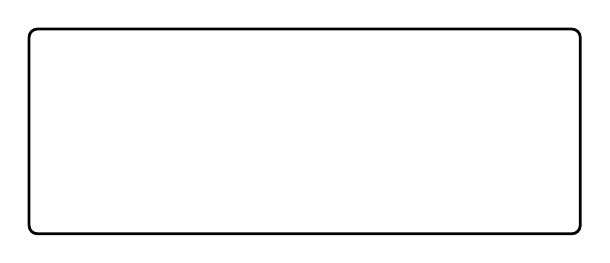
\begin{tikzpicture}\draw[line width=1pt,rounded corners=3pt] (0,0) rectangle (7,2.6); \end{tikzpicture}\end{center}
\end{puzzle}

\begin{puzzle}{Wrap}
A student wrote ``The model says everything is fine.'' Wrap it with a better claim. \wline[6cm]
\end{puzzle}

\begin{puzzle}{Design a test}
Say how you would find out whether your bike fits in the shed, using a model. \wline[6cm]
\end{puzzle}
\clearpage

\thispagestyle{fancy}
\subhead{Question record}
Write three more questions. Predict from the model, then check the real thing.\par\medskip
\renewcommand{\arraystretch}{3.0}
\begin{tabularx}{\linewidth}{|>{\sffamily\small\bfseries}p{3.2cm}|X|X|X|}
\hline
Question & Model says & Real thing & Match? \\ \hline
 & & & \\ \hline
 & & & \\ \hline
 & & & \\ \hline
\end{tabularx}

\vspace{8pt}
Which question could the model not answer? \wline[7cm]\\[10pt]
What would the model need to keep to answer it? \wline[5cm]\\[10pt]
Sketch the part of your model that answers your best question.\par\medskip
\begin{tikzpicture}\draw[ink!70,line width=1pt,rounded corners=3pt] (0,0) rectangle (11.4,5.2);\end{tikzpicture}
\clearpage
